\documentclass[12pt]{report}

\usepackage{fullpage}
\usepackage{amsmath,amssymb,bm,upgreek,mathrsfs}
\usepackage{algorithmic,algorithm}
\usepackage{graphicx,subcaption}
\usepackage{setspace}
\usepackage{color}
\usepackage{multirow}
\usepackage{alltt}
\usepackage{cancel}
\usepackage{listings}

\doublespacing

\DeclareMathOperator*{\argmax}{arg\,max}
\DeclareMathOperator*{\argmin}{arg\,min}

\newcommand{\N}{\mathcal{N}} \newcommand{\U}{\mathcal{U}}
\newcommand{\Poi}{{\text Poisson}} \newcommand{\Exp}{{\text Exp}}
\newcommand{\G}{\mathcal{G}} \newcommand{\Ber}{{\text Bern}}
\newcommand{\Lap}{{\text Laplace}} \newcommand{\btheta}{\boldsymbol{\theta}}
\newcommand{\bSigma}{\boldsymbol{\Sigma}}

\newcommand{\E}[1]{\mathbb{E}[#1]}
\newcommand{\Cov}[2]{\mathbb{C}\mathrm{ov}(#1,#2)}

\def\*#1{\mathbf{#1}} \newcommand*{\V}[1]{\mathbf{#1}}

%%%%%%%%%%%%%%%%%%%%%%%%%%%%%%%%%%%%%%%%%%%%%%%%%%%%%%%%%%%%%%%%%%%%%%

\begin{document}

\centerline{\it CS 477 HW \#11}
\centerline{Questions completed: All undergrad level questions in MATLAB}

\begin{enumerate}

\item[A1.] Implementing K-means clustering.

  In this section, the K-means clustering segmentations are shown. For the
  K-means stopping criterion, the approach of waiting until the clustering
  assignments do not change was chosen with a fallback max iteration number of
  200. Luckily, this did not have to be reached for any of the image
  segmentations. My thoughts on this are that the method we choose does not
  really matter since we are only working with trivial examples in this
  assignment. It is a good point however that for real world usage, you might
  have a break case if you know that bad starting point clusters were
  selected. The ideal solution in contrast is just to have enough computing
  resources so that you can keep the workflow as simple as possible.

  \newpage
  In Figure 1 below, the original sunset.tiff image, the K=5 segmentation, and
  K=10 segmentation are shown below.

  \begin{figure}[H]
    \centering
    \begin{subfigure}{0.48\linewidth}
      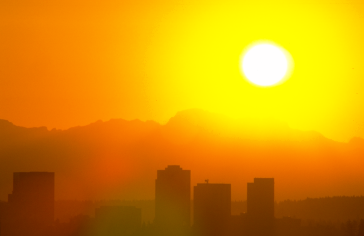
\includegraphics[width=\linewidth]{sunset.png}
      \caption{Original sunset.tiff image.}
    \end{subfigure}
    \begin{subfigure}{0.55\linewidth}
      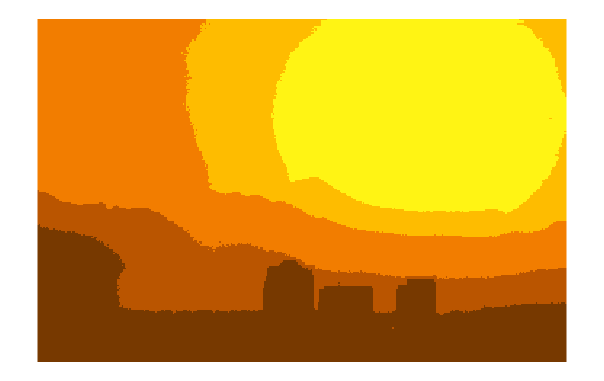
\includegraphics[width=\linewidth]{1a5.png}
      \caption{Segmentation with K=5.}
    \end{subfigure}
    \begin{subfigure}{0.55\linewidth}
      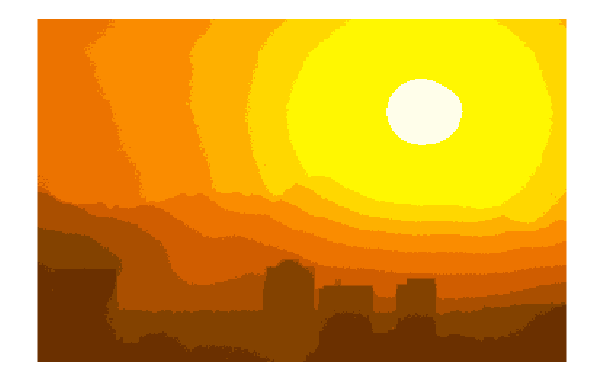
\includegraphics[width=\linewidth]{1a10.png}
      \caption{Segmentation with K=10.}
    \end{subfigure}
    \caption{Segmentation of sunset.tiff.}
  \end{figure}

  \newpage
  In Figure 2 below, the original tiger-1.tiff image, the K=5 segmentation, and
  K=10 segmentation are shown below.

  \begin{figure}[H]
    \centering
    \begin{subfigure}{0.48\linewidth}
      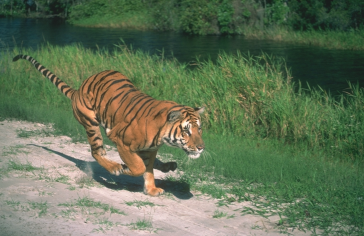
\includegraphics[width=\linewidth]{tiger-1.png}
      \caption{Original tiger-1.tiff image.}
    \end{subfigure}
    \begin{subfigure}{0.55\linewidth}
      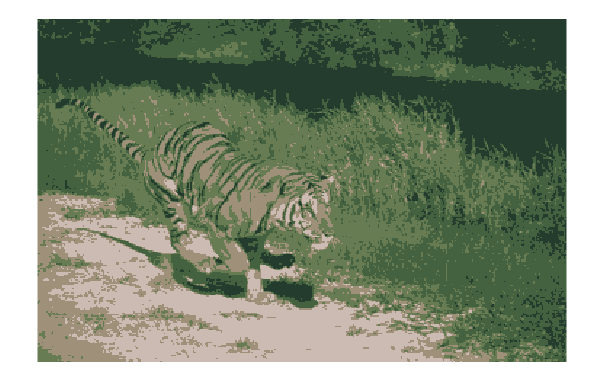
\includegraphics[width=\linewidth]{2a5.png}
      \caption{Segmentation with K=5.}
    \end{subfigure}
    \begin{subfigure}{0.55\linewidth}
      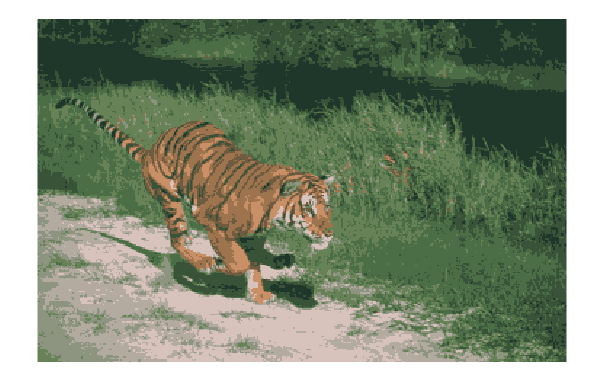
\includegraphics[width=\linewidth]{2a10.png}
      \caption{Segmentation with K=10.}
    \end{subfigure}
    \caption{Segmentation of tiger-1.tiff.}
  \end{figure}

  \newpage
  In Figure 3 below, the original tiger-2.tiff image, the K=5 segmentation, and
  K=10 segmentation are shown below.

  \begin{figure}[H]
    \centering
    \begin{subfigure}{0.48\linewidth}
      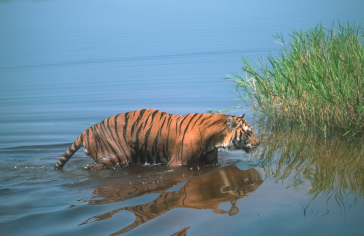
\includegraphics[width=\linewidth]{tiger-2.png}
      \caption{Original tiger-2.tiff image.}
    \end{subfigure}
    \begin{subfigure}{0.55\linewidth}
      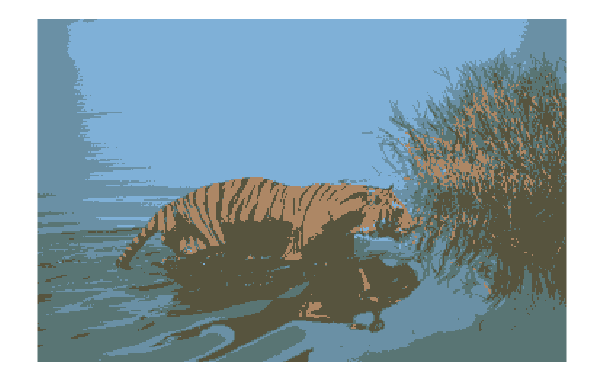
\includegraphics[width=\linewidth]{3a5.png}
      \caption{Segmentation with K=5.}
    \end{subfigure}
    \begin{subfigure}{0.55\linewidth}
      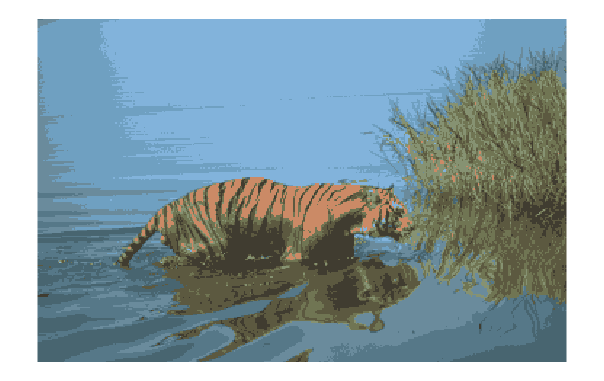
\includegraphics[width=\linewidth]{3a10.png}
      \caption{Segmentation with K=10.}
    \end{subfigure}
    \caption{Segmentation of tiger-2.tiff.}
  \end{figure}

\item[A2.] 5-dimensional feature vector.

  In Figure 4 below, segmentation using the specified 5-dimensional feature
  vector of \( (R,G,B,\lambda*X,\lambda*Y)\) is shown for the three images using
  \( \lambda=1\) and \( \lambda=10\) for \( K=10\) clusters.

  \begin{figure}[H]
    \centering
    \begin{subfigure}{0.48\linewidth}
      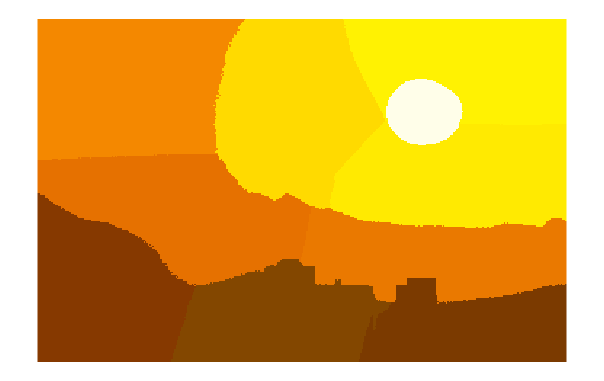
\includegraphics[width=\linewidth]{1b1.png}
      \caption{sunset.tiff with \( \lambda=1\).}
    \end{subfigure}
    \begin{subfigure}{0.48\linewidth}
      
\includegraphics[width=\linewidth]{1b10.png}
      \caption{sunset.tiff with \( \lambda=10\).}
    \end{subfigure}
    \begin{subfigure}{0.48\linewidth}
      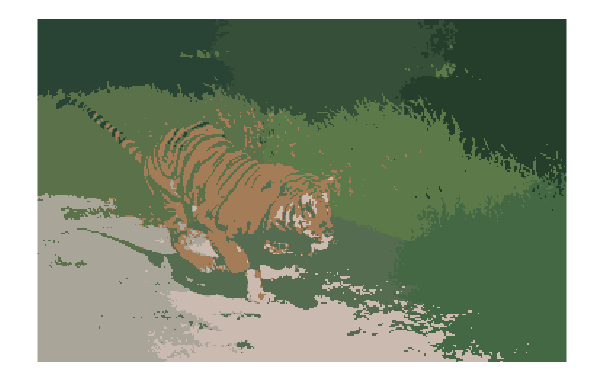
\includegraphics[width=\linewidth]{2b1.png}
      \caption{tiger-1.tiff with \( \lambda=1\).}
    \end{subfigure}
    \begin{subfigure}{0.48\linewidth}
      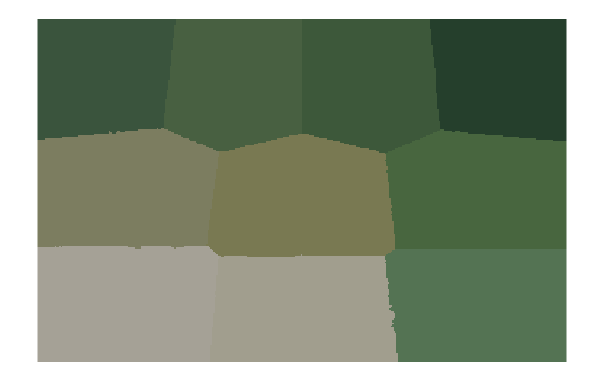
\includegraphics[width=\linewidth]{2b10.png}
      \caption{tiger-1.tiff with \( \lambda=10\).}
    \end{subfigure}
    \begin{subfigure}{0.48\linewidth}
      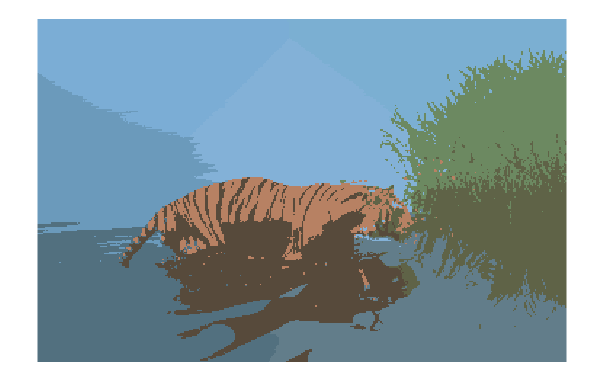
\includegraphics[width=\linewidth]{3b1.png}
      \caption{tiger-2.tiff with \( \lambda=1\).}
    \end{subfigure}
    \begin{subfigure}{0.48\linewidth}
      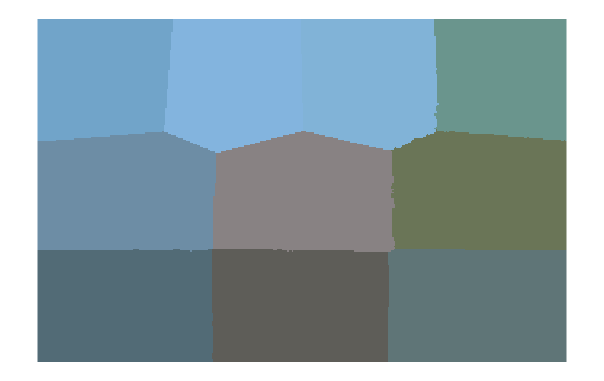
\includegraphics[width=\linewidth]{3b10.png}
      \caption{tiger-2.tiff with \( \lambda=10\).}
    \end{subfigure}
    \caption{Segmentation of images (K=10) with 5-dimensional feature vector.}
  \end{figure}

  Based on Figure 4 above, it appears that increasing \( \lambda\) which is the
  weight placed on the pixel position results in segmentation that is more
  sensitive to the position of the pixels. This is seen from the difference
  between the left and right images of Figure 4 for every row.

  \newpage
\item[A3.] Using texture features.

  Below in Figure 5, results for the three different feature vectors for each of
  the three images are shown. The parameters are \( W=10\times 10\) window size,
  \( K=10\) clusters, and \( \lambda=1\) as the pixel position
  weight. Additionally, the root mean squared value in the window \( W\) was
  taken instead of the mean squared value. All features in the feature vector
  were scaled to the range of 0 to 255.

  \begin{figure}[H]
    \centering
    \begin{subfigure}{0.3\linewidth}
      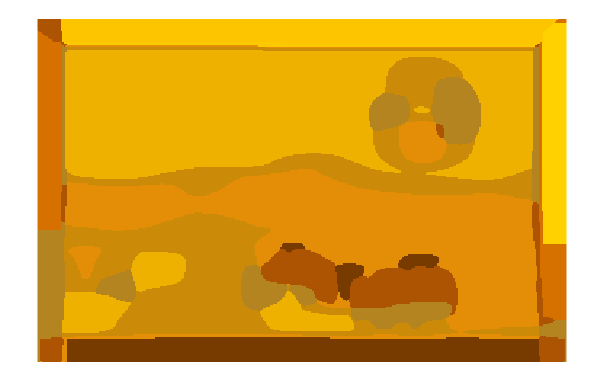
\includegraphics[width=\linewidth]{p1img1c.png}
      \caption{sunset w/ texture.}
    \end{subfigure}
    \begin{subfigure}{0.3\linewidth}
      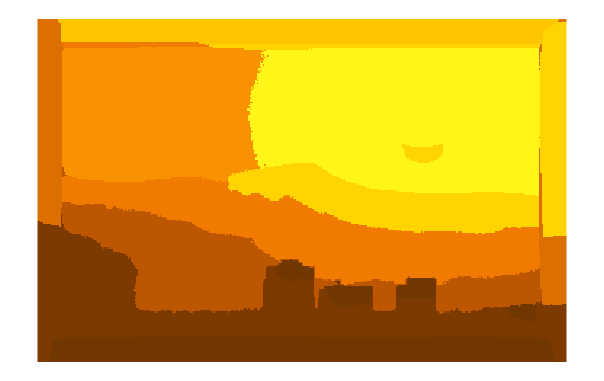
\includegraphics[width=\linewidth]{p2img1c.png}
      \caption{sunset w/ texture, rgb.}
    \end{subfigure}
    \begin{subfigure}{0.3\linewidth}
      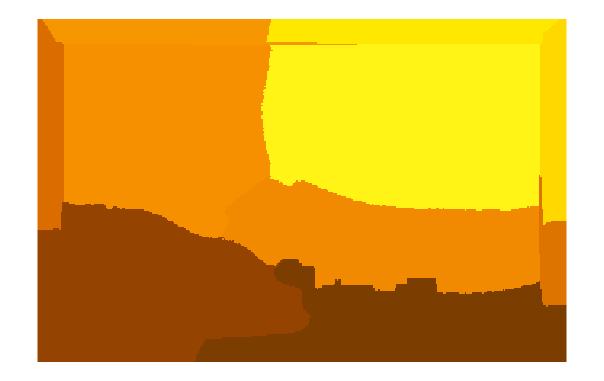
\includegraphics[width=\linewidth]{p3img1c.png}
      \caption{ texture, rgb, position.}
    \end{subfigure}
    \begin{subfigure}{0.3\linewidth}
      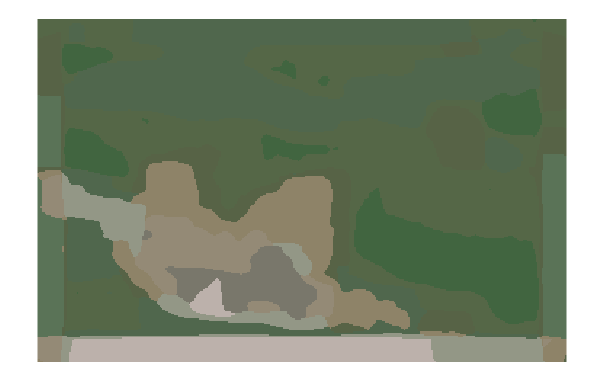
\includegraphics[width=\linewidth]{p1img2c.png}
      \caption{tiger-1 w/ texture.}
    \end{subfigure}
    \begin{subfigure}{0.3\linewidth}
      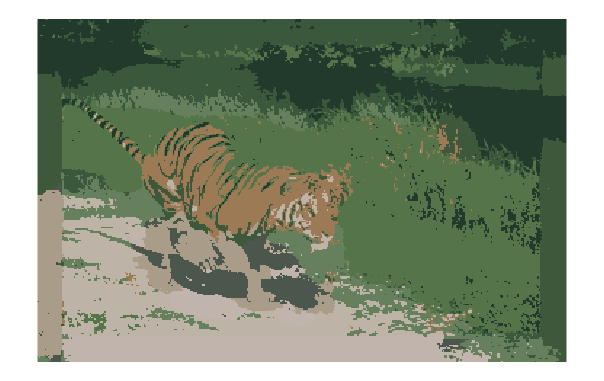
\includegraphics[width=\linewidth]{p2img2c.png}
      \caption{tiger-1 w/ texture, rgb.}
    \end{subfigure}
    \begin{subfigure}{0.3\linewidth}
      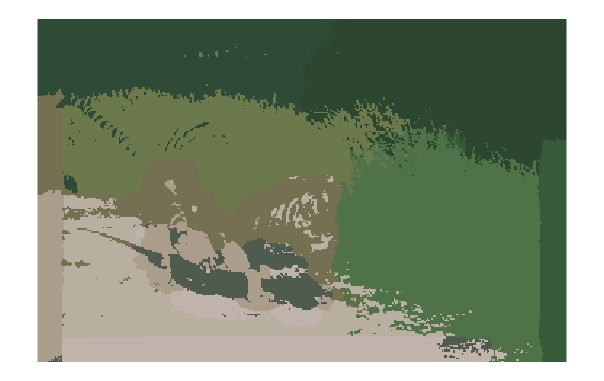
\includegraphics[width=\linewidth]{p3img2c.png}
      \caption{ texture, rgb, position.}
    \end{subfigure}
    \begin{subfigure}{0.3\linewidth}
      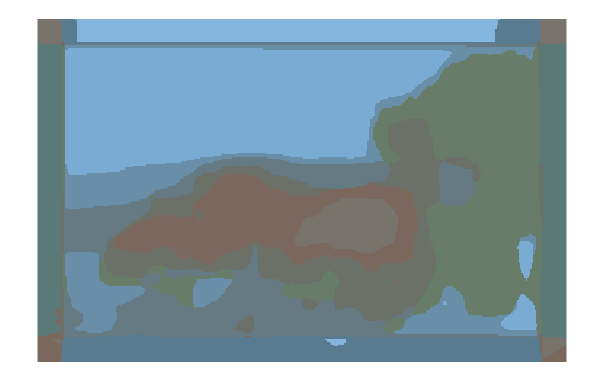
\includegraphics[width=\linewidth]{p1img3c.png}
      \caption{tiger-2 w/ texture.}
    \end{subfigure}
    \begin{subfigure}{0.3\linewidth}
      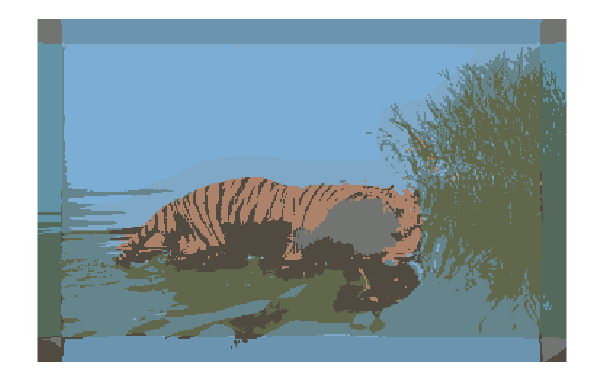
\includegraphics[width=\linewidth]{p2img3c.png}
      \caption{tiger-2 w/ texture, rgb.}
    \end{subfigure}
    \begin{subfigure}{0.3\linewidth}
      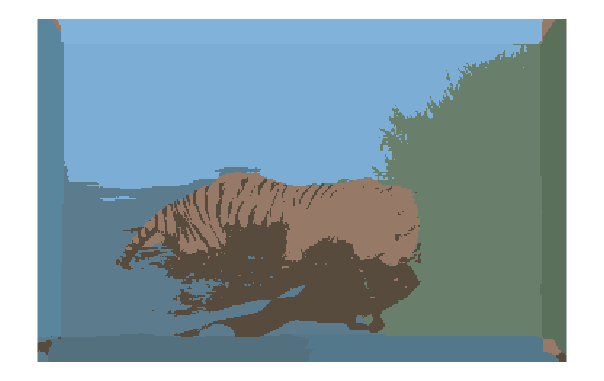
\includegraphics[width=\linewidth]{p3img3c.png}
      \caption{ texture, rgb, position.}
    \end{subfigure}
    \caption{Segmentation of images (K=10) with 5-dimensional feature vector.}
  \end{figure}

  From Figure 5 above, we can see that using just texture features alone (first
  column) gives an interesting segmentation that is better than just placing a
  high weight on position with RGB but worse than segmentation with RGB
  alone. Using texture features plus RGB (second column) also gives an
  interesting segmentation, but it seems that texture features corrupts more
  than helps segmentation that would have been done with just RGB. Finally,
  using texture features plus RGB plus position (third column) gives another
  interesting trio of segmentations, but it is perhaps worse than texture
  features plus RGB. For these images, it is perhaps better to cluster on just
  RGB alone as the groupings are mostly color-based, but for a different set of
  images that are mostly the same color, texture features may improve the
  segmentation.

  Another thing of note are the visual artifacts in the images around the
  borders that creates a second kind of border within the images. I ran into
  this issue in assignment 8, but ultimately I do not know where this exactly
  comes from. My best guess is that it arises from the convolution of the images
  used to average the texture features in the window \( W\) because I observed
  that the visual artifacts around the border changes as I change the window
  size, so perhaps it is just the way that I am convolving images in MATLAB that
  produces this unwanted visual artifact.

% \item[B1.] Finding the magnitude of the gradient using convolution.

%   Below in Figure 1, the magnitude of the gradient for the climber.tiff image is
%   shown.

%   \begin{figure}[H]
%     \centering \fbox{
%       \begin{minipage}{.8\linewidth}
%         \includegraphics[width=\linewidth]{b1.png}
%         \caption{The gradient magnitude image was generated in MATLAB using the
%           `conv2()' function to find the x and y gradients. The resulting
%           gradient matrix brightness was properly scaled to get a sensible image
%           as shown.}
%         \label{fig:b1}
%       \end{minipage}}
%   \end{figure}

%   First, the image was read into MATLAB, converted into grayscale, and then
%   casted into double values. Next, the finite difference kernels for the x and y
%   gradients were defined as `dx = [1 -1]' and `dy = [1; -1]', and convolution
%   was performed doing ``conv2(climber, dx, `same')'' (and same for dy) with the
%   third optional argument of `same' since we only want the central part of the
%   convolution that is the size of the image. Finally, once we have our x and y
%   gradients which are the two components of our gradient vectors, we can
%   construct the matrix of gradient magnitudes, also known as the edge
%   strength. Brightness scaling was done on the gradient matrix by dividing the
%   values of the matrix by the maximum value in the matrix times 255.

%   \newpage
% \item[B2.] Finding a threshold for the gradient magnitude.

%   In Figure 2 below, the image of the gradient magnitude with a set threshold is
%   shown.

%   \begin{figure}[H]
%     \centering \fbox{
%       \begin{minipage}{.8\linewidth}
%         \includegraphics[width=\linewidth]{b2.png}
%         \caption{In MATLAB, the gradient magnitude from Figure 1 was filtered so
%           that any gradient magnitude exceeding the threshold is set to white,
%           otherwise set to black.}
%         \label{fig:b2}
%       \end{minipage}}
%   \end{figure}

%   My attempt at finding a reasonable threshold to filter the gradient magnitude
%   was first finding the max, min, mean, and median of the values in the gradient
%   matrix so that I could get a feel for what I am working with. Upon inspecting
%   the values, I noticed that the mean was higher than the median which suggested
%   a right-skewed distribution. I opted to try out the mean as the threshold and
%   decided after comparing this mean threshold to other thresholds that the mean
%   of 18.5 for the gradient matrix threshold suffices. Anything above this mean
%   value was set to white (255), and anything below this mean value was set to
%   black (0) to produce Figure 2 above.

%   \newpage
% \item[B3.] Using convolution to smooth image.

%   Below in Figure 3, the surface map of the Gaussian kernel with \( \sigma=2 \)
%   is shown.

%   \begin{figure}[H]
%     \centering \fbox{
%       \begin{minipage}{.8\linewidth}
%         \includegraphics[width=\linewidth]{b3.png}
%         \caption{In MATLAB, a 13x13 Gaussian kernel with \( \sigma=2 \) was
%           created to use in convolution. The Gaussian kernel is displayed using
%           the `imagesc()' function which automatically scales up and color codes
%           our Gaussian kernel matrix.}
%         \label{fig:b3}
%       \end{minipage}}
%   \end{figure}

%   The Gaussian kernel defined as \( e^{-\frac{x^2+y^2}{2\sigma^2}} \) in the
%   lecture was created with sigma set at 2 pixels. Accordingly, the dimensions of
%   the kernel was computed as \( DIM = 2 * 3 * \sigma + 1 = 13\) to get a 13x13
%   kernel. This ensures that the distribution is centered within the kernel and
%   that we are capturing 99\% of the distribution in both directions. Truncating
%   the kernel at \( 3 \sigma \) maintains a balance of capturing most (99\%) of
%   the Gaussian spread while at the same time limiting the kernel size in order
%   to increase computational efficiency (smaller kernel size is better). The
%   Gaussian kernel was then scaled by dividing its values by the sum of its
%   values in order to get a kernel whose values summed up to 1. This scaling is
%   done so that when convolution is used with the Gaussian kernel to smooth the
%   image, the output image is displayable as shown next.

%   Below in Figure 4, Gaussian smoothing of the original climber.tiff image is
%   shown.

%   \begin{figure}[H]
%     \centering \fbox{
%       \begin{minipage}{.8\linewidth}
%         \includegraphics[width=\linewidth]{b4.png}
%         \caption{In MATLAB, the Gaussian kernel as previously described was used
%           to perform convolution using `conv2()' to smooth the original
%           climber.tiff image.}
%         \label{fig:b4}
%       \end{minipage}}
%   \end{figure}

%   To perform the smoothing through convolution with a Gaussian kernel as seen
%   above in Figure 4, the function `conv2()' was used with the inputs being the
%   original climber.tiff image, our Gaussian kernel, and again passing `same' as
%   the third parameter. We can see in Figure 4 that our image indeed has been
%   smoothed.

% \item[B4.] Blurring followed by edge detection.

%   Below in Figure 5, edge detection and binary threshold filtering were
%   performed on the blurred image as shown.

%   \begin{figure}[H]
%     \centering \fbox{
%       \begin{minipage}{.8\linewidth}
%         \includegraphics[width=\linewidth]{b5.png}
%         \caption{In MATLAB, edge detection and threshold filtering was done for
%           our newly smoothed image from Figure 4. The same MATLAB operations
%           were as described in parts B1 and B2 were used.}
%         \label{fig:b5}
%       \end{minipage}}
%   \end{figure}

%   When comparing the edge detection with threshold on the blurred image compared
%   to the edge detection with threshold on the original image as seen in B2
%   Figure 2, it appears that the edge lines are much thicker than before. Whether
%   that improved the edge detection quality or not, I cannot say, but the edge
%   detection produced in Figure 2 seemed like it sufficed while this new edge
%   detection seen in Figure 5 seems overkill in terms of the thickness of edge
%   boundaries.

%   \newpage
% \item[B5.] Combining blurring and edge detection into one filter.

%   In Figure 6 below, the climber.tiff image is displayed after going through a
%   combined blurring and edge detection filter.

%   \begin{figure}[H]
%     \centering \fbox{
%       \begin{minipage}{.8\linewidth}
%         \includegraphics[width=\linewidth]{b6.png}
%         \caption{In MATLAB, a combined blurring and edge detection kernel is
%           applied to the climber.tiff image. The Gaussian component for the
%           blurring was set to \( \sigma=4 \).}
%         \label{fig:b6}
%       \end{minipage}}
%   \end{figure}

%   The Gaussian kernel and the simple finite difference edge detection kernels
%   (one for x and one for y) were combined through convolution using
%   `conv2(gauss, edge, `same')' so that we have two newly combined kernels for
%   the x and y directions. The gradient matrix was computed and threshold
%   filtered the same way as in described in B1. The blurring and edge detection
%   convolutions were also performed separately to compare to our combined filter,
%   and the resulting image matched well with our combined filter result with the
%   observation that the combined filter had slightly better detection of edges
%   using the same threshold, so perhaps combining kernels is a more streamlined
%   process.

% \item[B6.] Re-implementing smoothing using 1D convolution.

%   To prove that the Gaussian blurring function is separable:

%   \[ f(x,y)=e^{-\frac{x^2+y^2}{2\sigma^2}} \]
%   \[ f(x,y)=e^{\frac{-x^2-y^2}{2\sigma^2}} \]
%   \[ f(x,y)=e^{-\frac{x^2}{2\sigma^2}-\frac{y^2}{2\sigma^2}} \]
%   \[ f(x,y)=e^{-\frac{x^2}{2\sigma^2}}e^{-\frac{y^2}{2\sigma^2}} \]
%   \[ Let \ g(x) = e^{-\frac{x^2}{2\sigma^2}},\ h(y)=e^{-\frac{y^2}{2\sigma^2}}\]
%   \[ Then, \ f(x,y)=g(x)h(y) \]

%   Thus, we have proven that Gaussian blurring is a separable function. This
%   means that convolution with \( f(x,y) \) is the same as a 1D convolution by
%   \( g(x) \) followed by a 1D convolution by \( h(y) \).

%   Following this method, separate 1D Gaussian vectors were created for the x and
%   y direction with \( \sigma=2 \) and applied to the climber.tiff using
%   ``conv2(X, Y, image, `same')'' where X and Y are the Gaussian vectors, image
%   is climber.tiff, and `same' is the parameter as described previously. The
%   resulting smoothing was the same result as Figure 4 in B3.

%   I expect two 1D Gaussian vector convolutions to be faster than the single
%   Gaussian distribution matrix that we have been using because the size of the
%   kernel directly reflects the amount of computation that is required for
%   convolution of an image. Each convolution operation involves `sliding' the
%   kernel over the image and performing the computations at each pixel, so I am
%   guessing that the computation complexity is \( O(i*j*k^2)\) for an image with
%   \( i\) rows, \( j\) columns, and a \( k*k\) Gaussian kernel. Since our
%   Gaussian kernel is separable as we have proven above, we can do two 1D
%   convolutions which reduces the computation complexity to
%   \( O(i*j*2*k) = O(i*j*k) \).

%   The speeds were tested by putting the two different convolutions in a loop of
%   10,000 iterations each. Separating the Gaussian kernel approach took 1.82
%   seconds while the Gaussian matrix took 7.04 seconds. It is hard to say from
%   this whether the exact time complexities I listed above holds for these two
%   approaches as there is an unknown constant number of operations and overhead
%   in calling and using the conv2() function, but the basic theory holds that
%   convolutions are faster for smaller kernels.

\end{enumerate}

\end{document}
